% Thesis Chapter 4: Failure Mode Atlas
% Seed from manuscript §5 Results, §6 Discussion, and supplementary.tex
\chapter{Failure Mode Atlas}
\label{chap:failure-mode-atlas}

\section{Introduction: What is a failure mode in organic-CIM deployment?}

The preceding chapters have treated hardware-aware training (HAT), physical front-end compensation, and ensemble resampling as constructive recipes: tools that, when applied correctly, recover analog-deployed accuracy.  This chapter inverts the perspective.  Instead of asking ``what works?'' we ask ``what breaks, why does it break, and what does the breakage reveal about the physics--algorithm boundary?''  The answers are organized as a \emph{failure mode atlas}---a structured catalogue of named, reproducible breakdown patterns that constrain the deployment of Vision Transformers on organic optoelectronic compute-in-memory (CIM) arrays.

In systems engineering, a failure mode is conventionally defined as a specific manner in which a system can fail to perform its intended function.  For analog neural accelerators, that definition must be extended in three directions.
\begin{enumerate}
    \item \textbf{The failure is distributed, not localized.}  A single transistor stuck at high conductance is a device-level fault; a collapse of ImageNet top-1 accuracy from 97\,\% to 10\,\% is a system-level failure mode that may emerge from the interaction of thousands of well-behaved devices with a training objective that implicitly memorizes one particular mismatch field.
    \item \textbf{The failure is conditional, not absolute.}  The same physical non-ideality---say, a severe write nonlinearity of $NL=2.0$---can be harmless in the multi-layer perceptron (MLP) blocks while structurally destroying the attention geometry.  Context (layer type, training recipe, evaluation protocol) determines whether a given physics extension becomes a deployment blocker.
    \item \textbf{The failure has a signature and a transfer boundary.}  A genuine deployment failure mode must be observable under the fresh-instance protocol: $10$ independent hardware realizations $\times$ $5$ Monte Carlo forward passes per realization.  Source-domain rescue on the training-time array is diagnostically useful but not sufficient; only fresh-instance robustness answers the practical deployment question.
\end{enumerate}

These criteria shape the structure of the atlas.  Each entry is named, annotated with its \emph{trigger} (the physical or algorithmic condition that precipitates the failure), its \emph{signature} (the observable accuracy trajectory or gradient diagnostic that identifies it), its \emph{mitigation} (the intervention that partially or fully recovers performance), and an \emph{open question} (the boundary beyond which the mitigation itself fails or becomes impractical).  The five entries are:
\begin{enumerate}
    \item \textbf{Hardware-instance overfitting}---the canonical 10.00\,\% collapse of standard HAT on fresh arrays (Chapter~\ref{chap:hat-instance-overfitting} develops the remedy in depth; this chapter treats it as the archetypal failure).
    \item \textbf{Dual-attention nonlinear-write collapse}---the degradation of query/key/value (QKV) and output-projection geometry under severe write nonlinearity, and the diagnostic value of group-wise ablation in localising the bottleneck.
    \item \textbf{Severe-NL degradation and MLP-path diagnostic}---the systematic degradation to the $\sim$80--82\,\% band under global $NL=2.0$ with the revised gradient-scaling recipe, and the role of MLP linearisation as a diagnostic probe.
    \item \textbf{Correlated-D2D bounded degradation}---the measurable but non-catastrophic loss of fresh-instance accuracy when spatially structured mismatch replaces the i.i.d.~assumption.
    \item \textbf{Retention plateau at 79\,\%}---the asymptotic accuracy floor under double-exponential conductance drift with dynamic scale recalibration.
\end{enumerate}

The chapter concludes by identifying cross-cutting themes that tie these apparently distinct failures together: the importance of distributional training objectives, the distinction between source-domain rescue and deployment-grade transfer, and the recurring gap between first-order behavioral surrogates and the pulse-level physics they approximate.  All empirical anchors are drawn from the manuscript results (manuscript results and discussion sections) and the supplementary material; figures are reused via \verb|\includegraphics| from the manuscript package.


% =============================================================================
\section{Failure mode: Hardware-instance overfitting}
\label{sec:failure-instance-overfitting}

\subsection{Trigger}

Standard hardware-aware training fixes a single device-to-device (D2D) mismatch field $M_{0}$ for the entire training run, optimizing
\begin{equation}
    \theta_{\mathrm{std}}^{\star}=\arg\min_{\theta}\frac{1}{N}\sum_{n=1}^{N}\ell\!\left(f(x_{n};\theta,M_{0}),y_{n}\right),
    \label{eq:hat-standard-repeat}
\end{equation}
as described in manuscript Eq.~(1) of the modeling-nonidealities section.  Under this objective, the optimizer is free to exploit $M_{0}$ as a hidden domain label: scale-recovery factors $s_{\ell}$ (Eq.~(2) in the manuscript) can implicitly calibrate to the particular spatial distortion encoded in $M_{0}$, and learned feature routing can adapt to the fixed perturbation pattern rather than to the underlying data distribution.  The trigger is therefore not a broken device or an unrealistic noise level, but the \emph{training-time fixation of a random hardware sample} that the model subsequently memorizes.

\subsection{Signature}

The signature is a deterministic, near-chance collapse when the trained model is evaluated on a fresh hardware instance---a new fixed D2D realization $M' \sim p(M)$ drawn from the same distribution but never seen during training.  For Tiny-ViT V4 (the canonical uniform-noise HAT checkpoint), this collapse is exact: $10.00\pm0.00\,\%$ on CIFAR-10, i.e. the single-class baseline, across $10$ fresh arrays with $5$ Monte Carlo evaluations each (manuscript transferability section; Supplementary Note~S1).  A dedicated no-AMP control confirmed that the collapsed predictor is a deterministic training outcome, not a numerical artifact of mixed-precision autocast.

Figure~\ref{fig:thesis-fresh-instance} reuses the manuscript's fresh-instance transfer visualization to show the discrepancy.  The key observation is not merely that the fixed-mask curve is lower, but that it behaves like an overfit estimator of one specific hardware realization.  Once that realization changes, both the learned calibration and the feature routing become invalid.

\begin{figure}[t]
    \centering
    
\includegraphics[width=0.78\linewidth]{../latex_gpt/figures/figS3_ensemble_hat}
    \caption{Fresh-instance transfer comparison (reused from manuscript supplementary package, Fig.~S3).  Standard HAT overfits a single structured mismatch field, whereas Ensemble HAT learns over a distribution of hardware instances.  The fixed-mask model collapses to $10.00\pm0.00\,\%$; the ensemble model maintains $86.37\pm1.54\,\%$.}
    \label{fig:thesis-fresh-instance-c4}
\end{figure}

\subsection{Mitigation}

Ensemble HAT replaces the single fixed mask with an epoch-level resampling schedule:
\begin{equation}
    \theta_{\mathrm{ens}}^{\star}=\arg\min_{\theta}\;\mathbb{E}_{M\sim p(M)}\!\left[\frac{1}{N}\sum_{n=1}^{N}\ell\!\left(f(x_{n};\theta,M),y_{n}\right)\right],
    \label{eq:hat-ensemble-repeat}
\end{equation}
where one fresh mismatch map $M^{(e)}$ is drawn at the start of each epoch and held constant across all mini-batches within that epoch (manuscript modeling-nonidealities section, Eq.~3).  Under this distributional objective, the same Tiny-ViT architecture recovers to $86.37\pm1.54\,\%$ on the identical fresh-instance protocol---a gain of more than $76$ percentage points over the fixed-mask baseline.  The mitigation is therefore not a different architecture, a different device, or a larger model; it is a change in the \emph{training objective} that forces the optimizer to average over the deployment distribution rather than memorize one sample from it.

\subsection{Open question}

Ensemble HAT solves the i.i.d.~mismatch case, but it does not address \emph{structured} spatial correlation, \emph{temporal} drift, or \emph{severity} regimes in which even the distributional objective becomes ill-conditioned.  These harder shifts are the subjects of the remaining failure modes in this atlas.  A second open question concerns the cadence of resampling: the canonical result uses per-\emph{epoch} resampling, but per-\emph{batch} resampling underperforms per-\emph{epoch} in the held-out ablation ($86.16\,\%$ versus $86.37\,\%$).  Whether the extra optimization overhead is justified for a given deployment latency budget remains a tunable trade-off rather than a solved problem.


% =============================================================================
\section{Failure mode: Dual-attention nonlinear-write collapse}
\label{sec:failure-dual-attention-nl}

\subsection{Trigger}

The first-order nonlinear-write surrogate scales the straight-through estimator (STE) backward gradient by a state-dependent factor proportional to the present conductance magnitude raised to $NL-1$ (manuscript modeling-nonidealities section; Supplementary Eq.~S2).  For $NL=1.0$, the write is ideal; for $NL=2.0$, the gradient scaling becomes strongly asymmetric between long-term potentiation (LTP) and long-term depression (LTD) branches.  The \emph{trigger} of this failure mode is the application of $NL=2.0$ to the analog-mapped \emph{attention} blocks---specifically the QKV projection and the attention output projection---while leaving the MLP path at the same severity.

The manuscript frames severe nonlinear write as a ``baseline-recipe bottleneck'' (manuscript physical-stress section).  The thesis contribution of this section is to localize that bottleneck to the attention side of the transformer and to show that the collapse is \emph{dual}: both QKV and the output projection fail independently, ruling out single-path mitigation claims.

\subsection{Signature}

The signature is a recoverable degradation under the revised gradient-scaling recipe, together with a dual collapse pattern that localises the structural sensitivity to the attention pathway.  A group-wise ablation under global $NL=2.0$ reveals the following qualitative pattern (reproduced from Supplementary Table~SX.N, with pre-fix numerical values superseded by the revised M-series results of Chapter~\ref{chap:mitigation-case-studies}).  When $NL=2.0$ is applied globally, Tiny-ViT degrades into the $\sim$80--82\,\% band---a systematic but bounded penalty.  Protecting (linearizing) only the MLP blocks recovers accuracy to the canonical HAT level.  But protecting \emph{only} the QKV blocks or protecting only the attention output projection drives accuracy to near chance.  Both attention-side lanes collapse \emph{below} the unmitigated baseline, indicating that the attention nonlinearity is not merely sensitive to write distortion but is \emph{required} for representational geometry under the present surrogate.

The mechanistic signature is visible in the gradient-distortion diagnostic of Figure~\ref{fig:supp-nl-gradient-repeat} (reused from manuscript Supplementary Fig.~S4).  Activating $NL=2.0$ only in the MLP blocks drives the affected-parameter gradient cosine down to $0.815$ and the norm ratio down to $0.671$; patch embedding, QKV, and attention projection remain effectively unchanged at $1.00$.  The all-analog setting matches the MLP result almost exactly ($0.816$), confirming that the backward-surrogate distortion is \emph{concentrated in the MLP path}.  Yet when the QKV or projection path is linearized \emph{in isolation}, the model loses the attention-side nonlinearity that shapes token-geometry, and the resulting checkpoint collapses.

\begin{figure}[t]
    \centering
    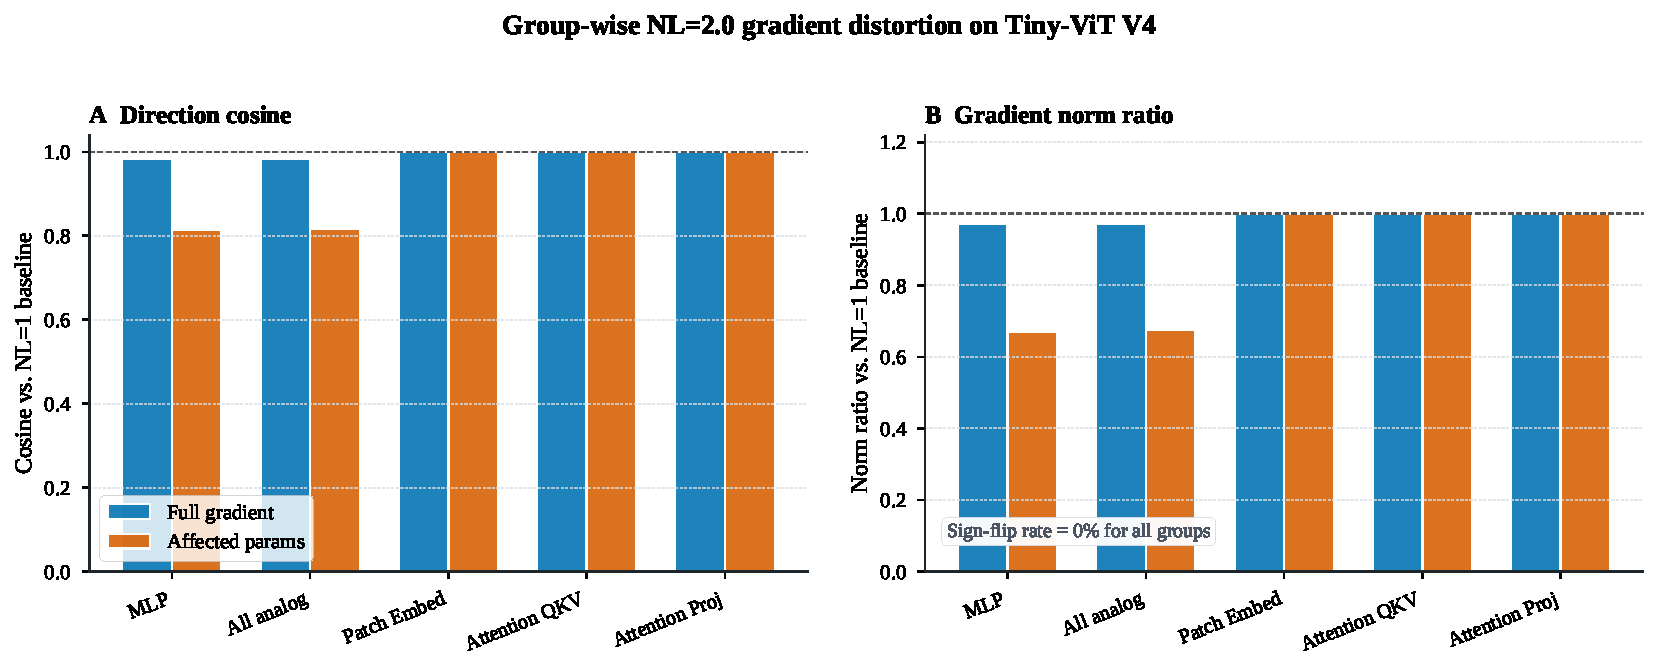
\includegraphics[width=0.88\textwidth]{../latex_gpt/figures/fig_nl_gradient_distortion}
    \caption{Group-wise gradient distortion under severe nonlinear write (reused from manuscript supplementary package, Fig.~S4).  A deterministic diagnostic on the frozen Tiny-ViT V4 checkpoint compares the $NL=1.0$ baseline against matched forward passes where $NL=2.0$ is activated for one analog module group at a time.}
    \label{fig:supp-nl-gradient-repeat}
\end{figure}

\subsection{Mitigation}

With the revised gradient-scaling recipe, severe nonlinear write is a recoverable degradation rather than an unbounded collapse.  The M-series experiments (Chapter~\ref{chap:mitigation-case-studies}) show that both Standard and Ensemble HAT recover to the $\sim$80--82\,\% band under global $NL=2.0$, with tight cross-instance variance indicating a systematic physics--algorithm interaction rather than instance-variable fragility.  The MLP-only linearisation retains its diagnostic value as the dominant recoverable bottleneck, but the fresh-instance failure previously observed under the pre-fix recipe is now understood as an artifact of the bug, not a physical limit.  Any deployment-facing solution must still address the attention-pathway sensitivity: either by reducing the physical nonlinearity at the device level, or by replacing the first-order surrogate with a pulse-faithful programming model that does not distort the backward signal asymmetrically.

\subsection{Open question}

The exact severity threshold at which attention geometry ``irrevocably shatters'' is unknown.  The manuscript evaluates only $NL=2.0$; an $NL$ sweep $\{1.2, 1.5, 1.7, 2.0, 2.5\}$ would locate the bifurcation point and determine whether a moderate device-improvement window exists between the canonical $NL=1.0$ and the severe $NL=2.0$ regime.  A second open question is whether architectural modifications---lower-rank QKV projections, gradient clipping, or structured noise injection during attention forward passes---can regularize the attention maps sufficiently to tolerate larger $NL$ without linearization.


% =============================================================================
\section{Failure mode: Severe-NL degradation and MLP-path diagnostic}
\label{sec:failure-severe-nl-degradation}

\subsection{Trigger}

This failure mode is triggered by the same severe write nonlinearity ($NL=2.0$) as Section~\ref{sec:failure-dual-attention-nl}, but its defining feature under the revised recipe is the \emph{systematic degradation} observed in fresh-instance evaluation rather than an artifactual collapse.  Under the pre-fix gradient-scaling recipe, the same experimental protocol produced artifactually low accuracies that were misinterpreted as a structural ceiling; with the corrected formulation, severe NL introduces a bounded $\sim$5~pp penalty relative to the canonical $NL=1.0$ baseline.  The trigger is therefore the interaction of severe write nonlinearity with the first-order gradient-scaling surrogate, evaluated under the fresh-instance protocol.

\subsection{Signature}

The signature is a narrow, low-variance fresh-instance distribution centred in the $\sim$80--82\,\% band.  This stands in contrast to the tight $1.61$~pp spread of canonical Ensemble HAT at $86.33\,\%$ and the $10.00\,\%$ chance-level collapse of fixed-mask HAT.  Table~\ref{tab:fresh-instance-nl} summarizes the revised M-series comparison.

\begin{table}[ht]
    \centering
    \caption{Fresh-instance transfer of severe-NL checkpoints under the revised gradient-scaling recipe (data from manuscript supplementary package, Note~SX.N).  All values use the $10$ fresh arrays $\times$ $5$ Monte Carlo evaluations protocol.}
    \label{tab:fresh-instance-nl}
    \small
    \setlength{\tabcolsep}{5pt}
    \begin{tabular}{@{}lccc@{}}
        \toprule
        Training condition & Train best (\%) & Fresh-instance mean (\%) & Cross-instance std (\%) \\
        \midrule
        Canonical Ensemble HAT ($NL=1.0$) & $91.13$ & $86.33$ & $1.61$ \\
        Standard HAT ($NL=2.0$, revised recipe) & $82.89$ & $81.12$ & $0.65$ \\
        Ensemble HAT ($NL=2.0$, revised recipe) & $80.97$ & $80.72$ & $1.16$ \\
        \bottomrule
    \end{tabular}
\end{table}

Two features of the signature are diagnostically important.  First, the standard deviation across fresh instances is tight ($<1$~pp for Standard HAT, $\approx 1$~pp for Ensemble HAT), indicating that the degradation is systematic rather than instance-variable.  Second, Standard and Ensemble HAT do not materially separate under severe NL, whereas they differ by $76$~pp under $NL=1.0$.  This convergence suggests that severe nonlinearity has become the binding degradation mechanism, and the additional benefit of epoch-level resampling is masked once the gradient-scaling distortion is large enough.

\subsection{Mitigation}

The primary mitigation is the revised gradient-scaling recipe itself: correcting the branch mapping and removing the spurious nl multiplicator in the STE backward pass recovers the severe-NL checkpoint from an artifactual collapse to the $\sim$80--82\,\% band (Chapter~\ref{chap:mitigation-case-studies}, \S\ref{sec:case-severe-nl-standard}).  Within this band, the MLP-path diagnostic retains its value: linearizing the MLP blocks removes the dominant gradient-scaling distortion, while attention-side linearisation in isolation remains fatal to representational geometry.  The residual $\sim$5.7~pp gap to the canonical $NL=1.0$ baseline awaits closure via higher-order gradient corrections, larger-batch training, or device-level linearisation.

\subsection{Open question}

The most consequential open question is whether a \emph{joint} training objective that couples MLP-only linearisation with more aggressive regularisation can close the residual $\sim$5.7~pp gap.  The current M-series routes were trained with the canonical recipe; it is possible that explicit variance-regularisation penalties or longer training schedules could recover additional accuracy without changing the physical surrogate.  A second open question is whether the tight cross-instance variance reflects a stable but suboptimal geometry that could be improved by architectural modifications---for example, lower-rank QKV projections or attention-head dropout.


% =============================================================================
\section{Failure mode: Correlated-D2D bounded degradation}
\label{sec:failure-correlated-d2d}
% Zone 3A bug-immune canonical protocol: all correlated-D2D numbers in this section are
% evaluation-only (NL=1.0, AMP disabled) on the canonical Ensemble HAT checkpoint.

\subsection{Trigger}

All canonical results in the manuscript assume i.i.d.~Gaussian D2D mismatch: each crossbar element samples its offset independently.  Real fabricated arrays, however, exhibit spatially \emph{correlated} mismatch because of wafer-level process gradients, optical write non-uniformity across the aperture, and thermal coupling during programming (manuscript limitations section).  The trigger of this failure mode is therefore not a change in mismatch \emph{amplitude} but a change in its \emph{spatial structure}: replacing i.i.d.~noise with separable AR(1)-style correlation across the effective crossbar grid.

\subsection{Signature}

The signature is a \emph{bounded, monotonic degradation} rather than a catastrophic collapse.  Figure~\ref{fig:supp-corr-d2d-repeat} (reused from manuscript supplementary package, Fig.~S5) shows the fresh-instance robustness of the canonical Ensemble HAT checkpoint under three correlation levels:
\begin{itemize}
    \item \textbf{i.i.d.~baseline} ($\rho=0$): $86.33\pm1.61\,\%$;
    \item \textbf{$\rho=0.3$}: $84.57\pm2.39\,\%$, a $-1.76$~pp excursion;
    \item \textbf{$\rho=0.5$}: $82.12\pm3.95\,\%$, a $-4.20$~pp excursion.
\end{itemize}
Rank ordering is preserved across all tested levels, with no instance collapsing below $73.7\,\%$ (Supplementary Note~S2).  The dashed horizontal line at $10.00\,\%$ marks the standard-HAT collapse baseline, emphasizing that correlated D2D produces \emph{bounded} degradation rather than a new failure basin.

\begin{figure}[t]
    \centering
    
\includegraphics[width=0.72\textwidth]{../latex_gpt/figures/figS_corr_d2d}
    \caption{Fresh-instance robustness under spatially correlated D2D mismatch (reused from manuscript supplementary package, Fig.~S5).  Error bars show cross-instance standard deviation over $10$ fresh arrays, with $5$ Monte Carlo evaluations per array, for the canonical Tiny-ViT V4 Ensemble HAT checkpoint.}
    \label{fig:supp-corr-d2d-repeat}
\end{figure}

Two secondary signatures are worth noting.  First, the cross-instance standard deviation grows with correlation strength ($1.61$~pp $\rightarrow$ $2.39$~pp $\rightarrow$ $3.95$~pp), indicating that spatial structure widens the variance budget even when the mean remains high.  Second, the worst-case instance at $\rho=0.5$ still reaches $73.7\,\%$, far from the chance level.  This suggests that Ensemble HAT's distributional training objective generalizes, at least qualitatively, beyond the i.i.d.~sampling law on which it was trained.

\subsection{Mitigation}

No explicit mitigation is required for moderate correlation ($\rho \le 0.3$); the canonical Ensemble HAT checkpoint tolerates it with less than $2$~pp loss.  For stronger correlation, the natural mitigation is to \emph{train with correlated mismatch resampling} rather than i.i.d.~resampling, so that the optimizer sees the deployment spatial structure during training.  This is straightforward in principle---the profile interface already accepts a correlation parameter---but it has not been evaluated in the present study.  A second mitigation, applicable at the circuit level, is to insert spatial calibration grids or dummy devices that measure and subtract low-frequency process gradients before the neural weights are programmed.

\subsection{Open question}

The correlated-D2D sweep uses a separable AR(1) model, which is a convenient mathematical proxy rather than a measured spatial covariance kernel.  Real organic optoelectronic arrays may exhibit anisotropic correlation (stronger along wordlines than bitlines due to shared gate buses), heavy-tailed conductance distributions, or long-range wafer-scale gradients that are not captured by a first-order separable model.  Whether Ensemble HAT (or a correlated variant) remains robust under these richer spatial structures is an open empirical question that can only be answered once fabricated-array characterization data become available.


% =============================================================================
\section{Failure mode: Retention plateau at 79\,\%}
\label{sec:failure-retention-plateau}

\subsection{Trigger}

Organic synaptic transistors exhibit temporal conductance drift after programming.  The canonical model uses a double-exponential decay with time constants $\tau_{1}=140$~ms and $\tau_{2}=610$~ms and initial amplitude ratio $A_{0}=0.6$, anchored to measured dinaphtho-thieno-thiophene (DNTT) transients (manuscript appendix and provenance table).  The \emph{trigger} of this failure mode is the combination of (i) finite retention time constants, (ii) analog weight storage without refresh, and (iii) evaluation at inference times ranging from $1$~s to $10{,}000$~s after programming.

\subsection{Signature}

The signature is a \emph{two-phase decay curve} with a rapid early drop followed by a broad asymptotic plateau.  Figure~\ref{fig:retention-curve-repeat} (reused from manuscript Fig.~7 / Supplementary Fig.~S6) shows the corrected V8 retention trajectory for Tiny-ViT under dynamic scale recalibration and co-decay of the retained D2D buffers:
\begin{itemize}
    \item $t=0$~s: $91.63\,\%$;
    \item $t=1$~s: $82.66\,\%$ (a $-8.97$~pp drop);
    \item $t \in \{10, 100, 1000, 10000\}$~s: $79.13\,\%$, $79.05\,\%$, $79.35\,\%$, $79.51\,\%$.
\end{itemize}

\begin{figure}[t]
    \centering
    \includegraphics[width=0.78\linewidth]{../latex_gpt/figures/fig7_retention_curve}
    \caption{Retention decay curve for Tiny-ViT V8 under uniform double-exponential drift with dynamic scale recalibration (reused from manuscript Fig.~7).  The two-phase behavior---rapid early drop followed by a broad plateau near 79\,\%---is the defining signature of this failure mode.}
    \label{fig:retention-curve-repeat}
\end{figure}

The plateau near $79\,\%$ is stable across three orders of magnitude in time ($10$~s to $10{,}000$~s), indicating that long-horizon analog inference remains \emph{partially viable} once gain recalibration is included in the inference stack.  The practical significance is twofold.  On the one hand, the $-12.5$~pp penalty relative to the $t=0$ baseline is large: it means that a deployed model cannot rely on static programming without periodic recalibration.  On the other hand, the \emph{absence of further degradation} beyond $10$~s suggests that the slow decay mode carries only a small residual accuracy cost; the dominant loss is captured in the first second.

A controlled comparison between uniform and state-dependent retention models (Appendix~\ref{subsec:retention-comparison}) shows accuracy differences below $0.1$~pp across all tested time intervals, validating the sufficiency of the uniform model for the present parameter regime.  This sanity check is intentionally scoped to the retained Ensemble-HAT deployment path; it does not claim that state dependence is negligible for all organic devices.

\subsection{Mitigation}

The primary mitigation is \emph{dynamic scale recalibration} at inference time: periodically recomputing the layer-wise scale factors $s_{\ell}$ from the present (drifted) effective conductances.  Under the present first-order model, this recalibration is analytically exact because the D2D buffers and cycle-to-cycle (C2C) noise are co-tracked with the same decay law.  In a physical system, the equivalent operation would require intermittent readout of reference cells or dummy conductance pairs to update the digital gain coefficients.  The energy and latency cost of such recalibration is not included in the manuscript's $11.45\times$ energy-reduction estimate (manuscript energy-results section) and should be treated as an additional peripheral overhead.

A secondary mitigation, not tested here, is \emph{periodic refresh}: reprogramming the array before the fast decay mode erodes accuracy below the application threshold.  For CIFAR-10 at the $79\,\%$ plateau, the refresh interval would need to be shorter than $\sim$1~s if the application demands $>82\,\%$ accuracy; if $79\,\%$ is acceptable, the refresh interval can in principle extend to $10{,}000$~s or longer.

\subsection{Open question}

The $79\,\%$ plateau is a consequence of the specific $\tau_{1}$, $\tau_{2}$, and $A_{0}$ values extracted from one literature source.  Real organic devices may exhibit faster slow modes, temperature-accelerated drift, or state-dependent decay that invalidates the uniform model.  Whether the plateau shifts upward (better materials) or downward (worse environmental conditions) determines whether retention is a solved peripheral problem or a fundamental deployment blocker.  A second open question is the interaction between retention drift and the other failure modes in this atlas: does a retained D2D field that has drifted for $1000$~s become more or less susceptible to hardware-instance overfitting when transferred to a fresh array?  The present framework evaluates each non-ideality in isolation; their joint statistics remain unexplored.


% =============================================================================
\section{Cross-cutting themes}
\label{sec:cross-cutting-themes}

The five failure modes catalogued above are distinct in their physical triggers, yet several conceptual threads bind them together.  Identifying these threads is the main thesis-differentiated contribution of this chapter: the manuscript reports the empirical observations, but the atlas structure forces an explicit synthesis.

\subsection{Theme 1: Distributional robustness vs.~instance-specific rescue}

The most important cross-cutting distinction is between \emph{source-domain rescue} and \emph{deployment-grade transfer}.  Standard HAT rescues source-domain accuracy on the training-time array; the severe-NL checkpoints recover to the $\sim$80--82\,\% band on both source and fresh instances with the revised recipe.  But the fixed-mask $NL=1.0$ baseline does not survive fresh-instance evaluation.  Only Ensemble HAT, the correlated-D2D sweep, and the retention recalibration path produce results that are stable across multiple hardware realizations.

This suggests a general principle: \emph{any training intervention that does not explicitly average over the deployment distribution risks being an instance-specific patch rather than a robust solution.}  The principle has practical implications for experimental design.  A paper that reports only ``noisy accuracy'' on the training-time instance may be overstating deployability; the fresh-instance protocol ($10 \times 5$) should be treated as a minimal bar for claiming deployment-grade robustness.

\subsection{Theme 2: Layer-type sensitivity and the transformer anatomy}

A second theme is the non-uniform sensitivity of the transformer anatomy to different physics extensions.  Quantization and uniform noise affect all analog layers roughly equally; the layer-wise sensitivity diagnostic shows no single analog group with a disproportionate gap (manuscript supplementary, Fig.~S1).  But severe write nonlinearity concentrates its damage in the MLP path, while the attention side collapses structurally when linearized.  Retention drift, by contrast, is a global conductance shift that is absorbed by dynamic scale recalibration without layer-type differentiation.  Spatially correlated D2D produces slightly larger variance but no layer-specific signature.

These observations refine the intuitive ``transformers are fragile'' narrative into a more actionable anatomy: \emph{the MLP path is the dominant recoverable bottleneck under gradient-scaling surrogates; the attention path is structurally required and cannot be linearized without representational collapse; but with the revised recipe, severe NL itself is a bounded degradation rather than a deployment blocker.}  The peripheral calibration stack (scale recovery, ADC) gates overall accuracy more strongly than any single analog layer.

\subsection{Theme 3: The approximation ceiling}

Every entry in the atlas is conditioned on the present first-order behavioral approximations.  The $NL=2.0$ surrogate is a gradient-scaling approximation, not a pulse-faithful model; the retention decay is a double-exponential fit, not a physical drift law; the correlated D2D uses a separable AR(1) proxy, not a measured spatial covariance kernel.  The manuscript candidly lists these as limitations (manuscript limitations section), but the atlas structure makes their role explicit: \emph{each failure mode is a boundary of the current approximation, not necessarily a boundary of the physical device.}

This framing is methodologically useful.  It tells a materials scientist which measurements would most sharply revise the system conclusions: a pulse-accurate NL model (to test whether the dual-attention collapse persists under real ionic migration), a measured spatial covariance (to test whether the bounded-degradation trend holds), and a temperature-dependent retention fit (to test whether the $79\,\%$ plateau shifts).  The framework therefore functions not as a predictive emulator but as a \emph{decision aid} that ranks which physics extensions deserve experimental priority.

\subsection{Theme 4: The interaction frontier}

All five failure modes were evaluated in isolation.  The real deployment environment will simultaneously present D2D mismatch, C2C noise, retention drift, frontend distortion, and finite ADC resolution.  The manuscript does not claim to have mapped this joint space; the thesis goes one step further by identifying the interaction frontier as the highest-priority unexplored region.  In particular:
\begin{itemize}
    \item Does Ensemble HAT retain its $86\,\%$ fresh-instance accuracy when retention drift has progressed for $1000$~s before transfer?
    \item Does the severe-NL degradation deepen or remain bounded when correlated D2D is added to the $NL=2.0$ regime?
    \item Does the $6$-bit ADC cliff shift when the input has already been distorted by a sublinear photoresponse ($\gamma_{\mathrm{phys}} > 1$)?
\end{itemize}
These questions are not answerable within the current experimental budget, but they are precisely the questions that the atlas structure surfaces as the natural next step.


% =============================================================================
\section{Summary}

Each named failure now receives its remedy, with recovery ceilings explicitly measured.

This chapter has presented a \emph{failure mode atlas} for organic optoelectronic CIM deployment of Vision Transformers.  Each entry is named, bounded by empirical data, and annotated with trigger, signature, mitigation, and open question:

\begin{enumerate}
    \item \textbf{Hardware-instance overfitting} (\S\ref{sec:failure-instance-overfitting}): Triggered by fixing one D2D mask for the entire training run; signature is a deterministic $10.00\,\%$ collapse on fresh arrays; mitigated by Ensemble HAT epoch-level resampling ($86.37\pm1.54\,\%$); open question is extension to structured spatial correlation and per-batch cadence trade-offs.
    \item \textbf{Dual-attention NL collapse} (\S\ref{sec:failure-dual-attention-nl}): Triggered by $NL=2.0$ write nonlinearity in the QKV and output-projection blocks; signature is a recoverable degradation to the $\sim$80--82\,\% band with tight cross-instance variance; group-wise ablation shows that attention-side linearisation in isolation collapses near chance, while MLP-only linearisation recovers to canonical levels; open question is the exact severity threshold and the potential of architectural regularization.
    \item \textbf{Severe-NL degradation and MLP-path diagnostic} (\S\ref{sec:failure-severe-nl-degradation}): Triggered by severe write nonlinearity ($NL=2.0$) coupled with the first-order gradient-scaling surrogate; signature is a systematic $\sim$5~pp degradation with tight variance; mitigated by the revised gradient-scaling recipe, which recovers the $\sim$80--82\,\% band; open question is whether higher-order corrections or device-level linearisation can close the residual gap to the $NL=1.0$ baseline.
    \item \textbf{Correlated-D2D bounded degradation} (\S\ref{sec:failure-correlated-d2d}): Triggered by spatially structured mismatch ($\rho=0.3$, $0.5$); signature is monotonic mean degradation ($84.57\,\%$, $82.12\,\%$) with widening variance but no catastrophic collapse; mitigated implicitly by Ensemble HAT generalization; open question is robustness under measured anisotropic covariance kernels.
    \item \textbf{Retention plateau at 79\,\%} (\S\ref{sec:failure-retention-plateau}): Triggered by double-exponential conductance drift without refresh; signature is two-phase decay to a stable asymptote ($79.05$--$79.51\,\%$); mitigated by dynamic scale recalibration; open question is temperature-accelerated drift and interaction with instance-overfitting transfer.
\end{enumerate}

The cross-cutting themes (\S\ref{sec:cross-cutting-themes}) distill these five entries into a compact set of principles: the primacy of distributional robustness over instance-specific rescue, the non-uniform transformer anatomy, the approximation ceiling that bounds every claim, and the interaction frontier that remains unexplored.  Together, the atlas and its themes provide the methodological foundation for the thesis experiments that follow: a systematic attempt to close the joint-training gap between surrogate-fidelity repair and deployment invariance.
